\documentclass[12pt,oneside]{report}

% \AddToHook{cmd/section/before}{\clearpage}

\usepackage[T1]{fontenc}

\usepackage{aas_macros}
\usepackage[letterpaper, top=1in]{geometry}
\usepackage{titlesec}

\titleformat{\chapter}{\normalfont\normalsize\centering}{\thechapter.}{1em}{}
\titleformat{\section}{\normalfont\normalsize\centering}{\thesection}{1em}{}
\titleformat{\subsection}{\normalfont\normalsize\centering}{\thesubsection}{1em}{}
% \titlespacing*{\chapter}{0pt}{0pt}{40pt} 
% \titlespacing*{\section}{0pt}{0pt}{20pt}
\renewcommand{\contentsname}{Table of Contents}
\AtBeginDocument{
      \renewcommand{\bibsection}{\chapter*{\bibname}}
  }

\usepackage{setspace}
\usepackage{booktabs}

\usepackage{etoolbox}% http://ctan.org/pkg/etoolbox
\makeatletter
% \patchcmd{<cmd>}{<search>}{<replace>}{<succes>}{<failure>}
\patchcmd{\@chapter}{\addtocontents{lof}{\protect\addvspace{10\p@}}}{}{}{}% LoF
\patchcmd{\@chapter}{\addtocontents{lot}{\protect\addvspace{10\p@}}}{}{}{}% LoT
\makeatother
\usepackage[tableposition=above]{caption}

\usepackage{amsmath}	% Advanced maths commands
\usepackage{txfonts}
\usepackage{hyperref}
\hypersetup{
    colorlinks=true,
    linkcolor=black,
    filecolor=black,
    urlcolor=black,
    citecolor=black,
    pdftitle={Thesis},
    pdfpagemode=FullScreen,
}
\urlstyle{same}
% \usepackage{amssymb}	% Extra maths symbols

\usepackage{graphicx}	% Including figure files
\graphicspath{{../figures/}} 
\usepackage{natbib}
\usepackage[nottoc,numbib]{tocbibind}

\usepackage{isotope}
% \usepackage[titles]{tocloft} % fig titles
% \renewcommand{\cftfigpresnum}{\figurename\enspace}
% \setlength{\cftfignumwidth}{5em}
% \renewcommand{\cfttabpresnum}{\tablename\enspace}
% \setlength{\cfttabnumwidth}{5em}


\pagestyle{plain}
\counterwithout{figure}{chapter}
\counterwithout{table}{chapter}
\counterwithout{equation}{chapter}


\defcitealias{cristallo+11}{C11}
\defcitealias{cristallo+15}{C15}
\defcitealias{ventura+13}{V13}
\defcitealias{karakas10}{K10}
\defcitealias{KL16}{KL16}
\defcitealias{karakas+18}{K18}
\defcitealias{james+21}{J21}



\newcommand{\JJ}{\citetalias{james+21}}
\newcommand{\cristallo}{\citetalias{cristallo+11}+\citetalias{cristallo+15}}
\newcommand{\karakas}{\citetalias{karakas10}}
\newcommand{\kl}{\citetalias{KL16}+\citetalias{karakas+18}}
\newcommand{\ventura}{\citetalias{ventura+13}}

\newcommand{\VICE}{\texttt{VICE}}
\newcommand{\caah}{[C/Mg]-[Mg/H]}
\newcommand{\caafe}{[C/Mg]-[Mg/Fe]}

\newcommand{\zoo}{\ensuremath{Z/Z_{\sun }}}
\newcommand{\Ycc}{\ensuremath{y_{\rm C}^{\rm CC}}}
\newcommand{\Yct}{\ensuremath{y_{\rm C}}}
\newcommand{\Yoc}{\ensuremath{y_{\rm Mg}^{\rm CC}}}
\newcommand{\Ycagb}{\ensuremath{y_{\rm C}^{\rm AGB}}}
\newcommand{\sun}{\ensuremath{\odot}}


\newcommand\T{\rule{0pt}{2.6ex}}       % Top strut
\newcommand\B{\rule[-1.2ex]{0pt}{0pt}} % Bottom strut
\newcommand{\possesivecite}[1]{\citeauthor{#1}'s \citeyearpar{#1}}
\newcommand{\alp}{$\alpha$}

\newcommand{\citetjack}{Roberts et al.~(2023, in prep.)}
\newcommand{\citepjack}{(Roberts et al.~2023, in prep.)}
\newcommand{\citealtjack}{Robert et al.~2023, in prep.}

\newcommand{\about}[1]{${\sim} #1$}

\setcitestyle{aysep={}} 
\setcitestyle{notesep={; }} 



\title{Carbon Nucleosynthesis}
% The list of authors, and the short list which is used in the headers.
% If you need two or more lines of authors, add an extra line using \newauthor
\author{Daniel A. Boyea}

% These dates will be filled out by the publisher
\date{\today}

\pagenumbering{roman}

\begin{document}

%\doublespacing


\begin{titlepage}
   \begin{center}
       \vspace*{5\baselineskip}
       \textbf{The Galactic Chemical Evolution of Carbon}\\
       Implications for Stellar Nucleosynthesis\\
       \vspace*{3\baselineskip}
        Undergraduate Research Thesis\\
       \vspace*{3\baselineskip}
    Presented in partial fulfillment of the requirements for graduation \textit{with research distinction in Astronomy and Astrophysics} in the College of Arts and Sciences of The Ohio State University\\
       \vspace*{3\baselineskip}
        by\\
       \vspace*{3\baselineskip}
       {Daniel Alexander Boyea}\\
       \vspace*{3\baselineskip}
       The Ohio State University\\
       April 2023\\
       \vspace*{3\baselineskip}
       Project Advisor: Professor David H. Weinberg, Department of Astronomy \\
       James W. Johnson 
       \vfill
   \end{center}
\end{titlepage}



% Abstract of the paper
\chapter*{Abstract}
\addcontentsline{toc}{chapter}{Abstract}
% context
Stellar evolution models provide uncertain predictions for elemental yields due to uncertainties in stellar physics.
% aims
Here, I constrain the nucleosynthetic yields of C using multizone Galactic chemical evolution models.
% results
By matching the slopes of the \caah\ and \caafe\ relationships in a sample of APOGEE subgiant stars, I find that CCSNe and AGB stars contribute \about{80\%} and \about{20\%} of total C production respectively.
% 
To also match the normalization of the trends, I estimate the CCSNe C/Mg yield ratio $\Ycc/\Yoc = 1.57 + 0.59 \left(Z/Z_\odot\right)$, which explains the \caah\ trend when including the AGB C contribution.
%
Variations in the star formation history only slightly impact the low [Mg/Fe] tail of the [C/Mg]-[Mg/Fe] relation. However, most of the scatter in the \caah\ distribution can be attributed to measurement errors and radial migration. 
% 
Due to the degeneracy between the normalization of elemental yields and the strength of mass-loading in Galactic outflows, I constrain only the {\it relative} yield of C and Mg from a simple stellar population and the metallicity dependence thereof. While measurements of gas-phase C abundances are challenging, my model is broadly consistent with the [C/O]-[O/H] trend observed in compiled literature measurements.


\chapter*{Acknowledgements}
\addcontentsline{toc}{chapter}{Acknowledgements}

James Johnson, for guiding me through this project and through my last year of undergraduate. Your feedback at every step of the process has been invaluable.
Wayne Schlingman, for everything you do for everyone. You are the glue holding together our department. David Weinberg and Jennifer Johnson, for listening to my earlier drafts of this work and providing excellent suggestions.

I also would not have made it here without all the support of my friends and family. Eric, even across the country, you have always been a point of support and stability, and I am always happy to be around you. Anya, you are a wonderful friend and I cannot thank you enough for your support this year. 
I love so many people in our department who have just been friends and have positive support: Kaia, Maria, Autumn, Simon, Mary, Aaliyah, Sanskruti, Alyssa, Harrison, Denis, and so many others. 
Finally, I thank my family for supporting me through a challenging year, and Arya for being such a loveable doodle.

%% Lists

\tableofcontents
\listoffigures
\listoftables
\newpage
\pagenumbering{arabic}

%%%%%%%%%%%%%%%%%%%%%%%%%%%%%%%%%%%%%%%%%%%%%%%%%%

%%%%%%%%%%%%%%%%% BODY OF PAPER %%%%%%%%%%%%%%%%%%

\chapter{Introduction}

Galactic chemical evolution (GCE) aims to understand the chemical and star formation histories of galaxies. At the core of GCE models are stellar yields---the amount of each chemical element stars produce (or destroy). Each element is produced in different amounts by different stars, leaving traces of the Galaxy's evolutionary history. Through \textit{Galactic Archeology}, we can reconstruct the history of our galaxy by investigating clues left behind in stars.

Here, I aim to understand C enrichment---where it is produced and how its abundances evolve over time. C is unique nucleosynthetically, one of few light elements (along with N) produced in asymptotic giant branch (AGB) stars \citep[e.g.][]{jennifer19, KL14}. C and N are well-studied elements since they are easy to observe in stellar spectra, even at the lowest metallicities \cite[e.g.][]{fabbian+09, nissen+14, lambert81, laird85, lambert86}. Additionally, C and N are used as age indicators in red giant branch stars \citep{martig16, MG15, hasselquist19, vincenzo+21}.

Gas-phase [C/O] ratios---observed in very low metallicity, high redshift damped Lyman-alpha systems (DLAs)---decrease with increasing [O/H] \citep{FN15, cooke+17}. Then, [C/O] increases above $\rm [O/H] \approx -1$ (\citealt{berg+19}; see discussion in \S\ref{sec:gas}).
While we know C is produced in AGB stars and core-collapse supernovae (CCSNe), we still have a limited understanding of the magnitude and metallicity-dependence of each process.


Despite their central role in GCE models, nucleosynthetic yields predicted by stellar evolution models are rife with uncertainties. The production rates of elements in stars are shaped by poorly understood processes, including mass loss, opacity, nuclear reaction rates, rotational mixing, and convection \citep{KL14,ventura+13, LC18}.
Changes in massive stars' explodability also introduce further variation and uncertainty in population-averaged yields \citep{emily+21}.

GCE models typically use unmodified nucleosynthetic predictions and attempt to create models matching observations by varying the star formation history (SFH) and other evolutionary parameters. Here, I introduce C yields as an additional free parameter, determining which yield prescriptions reproduce Galactic abundance trends.
\cite{james+23} examined similar GCE models of N, an element whose production is closely related to C. \cite{james+23} found that trends in N and O abundances can be explained by the metallicity dependence of relative N and O yields. Here, I extend their models to C and show that similar constraints on C and O relative yields can be obtained from observed abundance ratios. Additionally, I assess which yield prescriptions reproduce Galactic abundance trends while assessing the impact of GCE model assumptions, such as SFH and outflow mass loading.

Accurate determination of stellar birth abundances for C and N is challenging. When a star enters the red giant branch (RGB), material from the CNO-processed core is mixed with the envelope in first dredge up (FDU), enhancing N and depleting C \citep{iben67, vincenzo+21,KL14}. Measurements of these evolved stars'  atmospheres will no longer reflect their birth abundances.  Additionally, gas-phase measurements of C are extremely limited as C lacks strong lines in HII regions \citep{skillman+20}.

To this end, I use a sample of subgiant stars from APOGEE \citep{apogee17}. According to stellar evolution theory and observations \citep{gilroy89, korn+07, lind+08, souto+18, souto19}, these stars have not yet experienced FDU but have well-mixed photospheres. Their photosphoric abundances should thus represent their birth composition.  In Fig.~\ref{fig:subgiants}, I plot this sample, selected by the criteria in Roberts et al. (2023, in prep; see Appendix \ref{sec:jack}). These empirical results contain information on the relative C and Mg yields, which I use later in this work.

\begin{figure}[htp]
    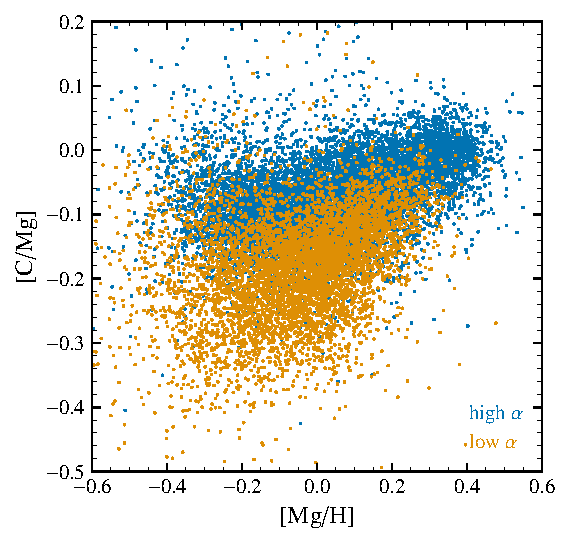
\includegraphics{subgiants_mgh.pdf}
    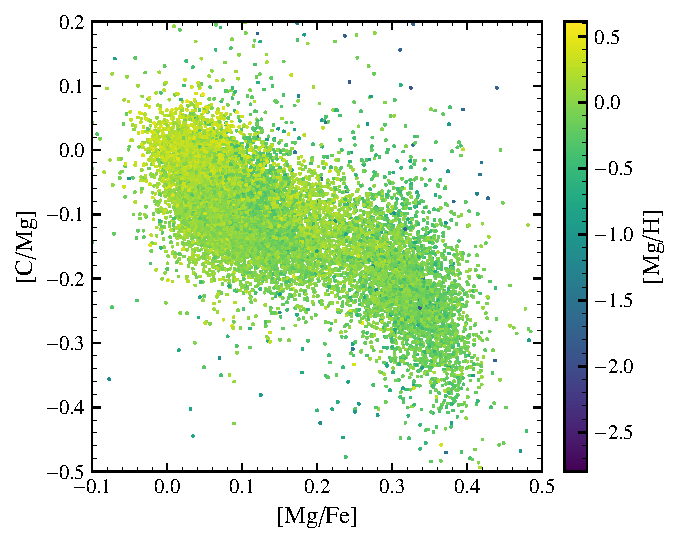
\includegraphics{subgiants_mgfe.pdf}
    \caption[APOGEE Subgiants]{The [C/Mg] ratio against [Mg/H] (top) and [Mg/Fe] (bottom) for the \citetjack~sample of APOGEE subgiants. On the top, I plot high and low-$\alpha$ stars in blue and orange, using the separation defined in Equation \ref{eq:high_alpha}. On the bottom, I color-code stars according to their [Mg/H] abundance.}
    \label{fig:subgiants}
\end{figure}


\chapter{Nucleosynthesis}

Theoretical models of stellar nucleosynthesis provide the starting point of this investigation. I focus on three primary nucleosynthetic pathways: asymptotic giant branch (AGB) stars, core-collapse supernovae (CCSNe), and type Ia supernovae (SNe Ia). Each process has unique timescales and yields, traceable through the tools of GCE. I compare C, produced in CCSNe and AGB stars, to Mg and Fe as tracers of CCSNe and SNe Ia respectively.

When a single stellar population (SSP) forms, CCSNe are the first enrichment event. CCSNe  explode within $\lesssim 40$ Myr, providing light elements (C, O, and Mg) and heavier elements (Fe and beyond). Metallicity-independent yields from CCSNe are the only statistically significant source of O and Mg ($\alpha$ elements). Next, low-mass stars begin to reach the end of their lives. By shedding their outer layers, AGB stars are important sources of C, N, and neutron capture elements.  Finally, white dwarfs explode, releasing Fe and other iron-peak elements.


For an element X and star with mass $M$, the stellar yield $\tilde{y}$ is defined as the net production of X relative to $M$, or
\begin{equation}
    \tilde{y}_{\rm X} = \frac{M_{\rm X,\ ejected} - Z_{0, X} M_{\rm ejected}}{M}   
\end{equation}
where $M_{\rm ejected}$ and $M_{\rm X, ejected}$  are the total ejected mass of the envelope and the element X, respectively. For example, if a 1 $M_\odot$ star has $\tilde{y}_{\rm C} = 10^{-3}$, then the star will add $10^{-3}\ M_\odot$ of C to the interstellar medium (ISM). 
Although per-star yields are necessary to compute AGB star enrichment rates in GCE models, IMF-averaged\footnote{IMF: Initial Mass Function} yields are useful in interpreting their predictions. For a yield $y$ from a star of mass M and initial metallicity $Z$, the IMF-averaged yield is given by 
\begin{equation} \label{eq:imf-yield}
    y_{\rm X}(Z) = 
    \int_{M_{\rm min}}^{M_{\rm max}} 
    \tilde{y}_{\rm X}(M, Z)
    \frac{dN}{dM}  \ dM
\end{equation}
where ${dN}/{dM}$ is the normalized IMF, and $M_{\rm min}$ and $M_{\rm max}$ are the minimum and maximum mass of stars, which I take to be $0.08 M_{\sun}$ and $100 M_{\sun}$ respectively. For AGB stars, the yields are truncated above 8 $M_{\odot}$. 
To calculate the IMF-weighted net yields, I use the Versatile Integrator for Chemical Evolution code (\VICE\footnote{\VICE~is available at \url{https://github.com/giganano/VICE}}).

To focus on C yields, I adapt the yield choices of other elements from \citet{james+21, james+23}.
Table \ref{tab:fiducial_mod} contains my fiducial yields, in units of a SSP's birth mass.
Also following \citet{james+21, james+23}, I take the SNeIa delay time distribution to be a
$t^{-1.1}$ power-law suggested by the observations of \citet{maoz+12}.


\begin{table}
	\centering
    \caption[Fiducial Model]{Yields for the fiducial model in units of SSP birh mass. See \S\ref{sec:agb} for the definition of C11.}
	\label{tab:fiducial_mod}

	\begin{tabular}{l l l l}
		\toprule
        Element & $\Ycc$ & $\tilde{y}^{\rm AGB}$ & $y^{\rm SNe Ia}$ \\
		\midrule
        C & $0.0028 + 0.001(Z/Z_\odot)$ & $2.9\times{\rm C11}$ &  0 \\
        Mg & 0.00185 & 0 & 0 \\
        Fe & 0.0012 & 0 & 0.00214 \\
        N & 0.00072 & $9\times10^{-4}(Z/Z_\odot)M$ & 0\\
		\bottomrule
	\end{tabular}
\end{table}

\section{Asymptotic Giant Branch Stars}\label{sec:agb}


An AGB star is a low mass ($\lesssim 8 M_{\sun}$) star during its final phase of evolution.  In an AGB star, two competing processes determine the outcome of C production: third dredge up (TDU) and hot bottom burning (HBB).  TDU accompanies thermal pulses in AGB stars. During a TDU event, material from the CO core is mixed with material exposed to partial He-shell burning, increasing C and O abundances in the envelope \citep{KL14}. If this envelope is lost during the AGB phase, then C yields are enhanced.
HBB is the activation of proton capture reactions, and the CNO cycle%
\footnote{The CNO (I) cycle is
\isotope[12]{C}(p, $\gamma$)
\isotope[13]{N}($\beta^+ \nu_e$)
\isotope[13]{C}(p, $\gamma$)
\isotope[14]{N}(p, $\gamma$)
\isotope[15]{O}($\beta^{+}\nu_e$)
\isotope[15]{N}(p, \alp)
\isotope[12]{C}.
 Other minor branches of the CNO cycle are of minor importance to C yields
 \citep{solar-fusion}.
}
at the base of the convective envelope. Because the $^{14}$N(p, $\gamma$) proton capture is the slowest component of the CNO cycle \citep{solar-fusion}, the CNO cycle converts nearly all \isotope[12]{C} into \isotope[14]{N}.
As a result, when both TDU and HBB occur, \isotope[12]{C} yields are lowered (see discussion in \citealt{james+23} and \citealt{ventura+13}).

In this work, I explore four different sets of AGB star yield tables from literature, providing well-sampled grids in metallicity and mass for use in chemical evolution models. 
\begin{itemize}
    \item C11: \citet{cristallo+11, cristallo+15}
    \item K10: \citet{karakas10}
    \item V13: \citet{ventura+13,ventura+14,ventura+18, ventura+20}
    \item K16: \citet{KL16} \citet{karakas+18}
\end{itemize}
I use C11 table, amplified by a factor of 2.9, as the fiducial AGB yield.

Fig.~\ref{fig:y_agb} compares the AGB C yield $\tilde{y}_\text{C}^\text{AGB}(M, Z)$ for each model I consider. 
The yields may be negative if a star returns material to the ISM with a lower C abundance than the material the star was formed from.
Most models agree on the qualitative shape of the net fractional AGB C yield---% 
stars with masses between \about{2~M_\odot} and \about{4~M_\odot} have the highest fractional C yields, with the mass of the peak increasing and overall yields decreasing with increasing $Z$.  High mass, high $Z$ stars destroy \isotope[12]{C} because they experience both TDU and HBB, but HBB is much more efficient.

In Fig.~\ref{fig:agb-ssp}, I plot the total production of C by AGB stars in a SSP at an age $t$. 
Effectively, this is equivalent to integrating Eq.~\ref{eq:imf-yield} down to $M_{to}$, the turnoff mass for time $t$.
({In our model, the mass-lifetime relation is
$\log \tau_M = 1.02 - 3.57\log M + 0.90 \left(\log M\right)^2$,
where $\tau_M$ is in Gyr,
from \citealt{larson74}.})
As the mass range $2\lesssim M \lesssim 4$ is most important for C production, about half of C production occurs before \about{1} Gyr, similar to SNe Ia Fe. 
K10 and K16 weight C production more heavily towards massive stars resulting in a faster enrichment delay time, whereas the C11 and V13 models predict a slightly longer timescale of \about{1} Gyr, but little to no C is produced more than 2 Gyr after a star formation event. This is in contrast to Fe whos production lasts up to 10 Gyr after a star formation event. As shown in the right panel of Fig.~\ref{fig:agb-ssp}, with increasing $Z$, C enrichment occurs earlier, and C destruction in low-mass stars leads to a declining C abundance at late times.
    

\begin{figure}
    \centering
 	    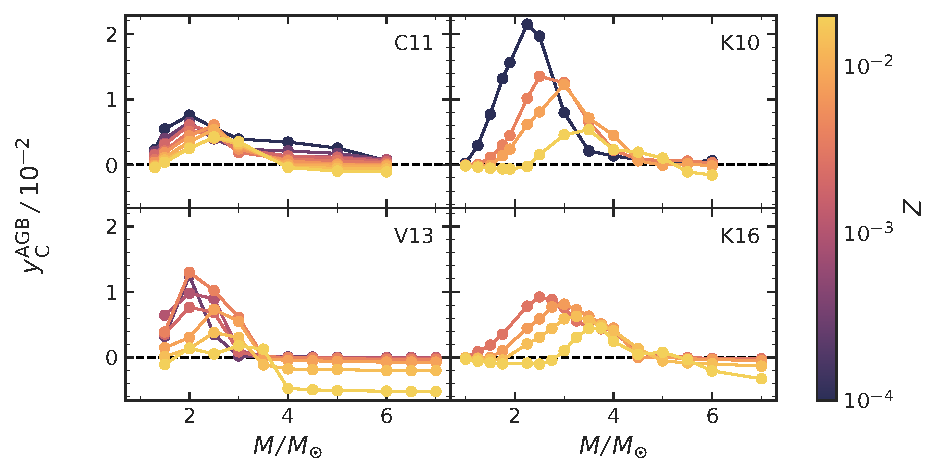
\includegraphics[scale=1]{agb_yields.pdf}
        \caption[AGB C yields]{The net fractional AGB C yield  plotted as a function of initial stellar mass $M$ and color-coded according to metallicity. The black dashed line shows $\tilde{y}=0$ for reference. Each panel represents yields from one of four AGB models: C11, K10, V13, K16 (see \S \ref{sec:agb}). }
        \label{fig:y_agb}
\end{figure}
\begin{figure}
    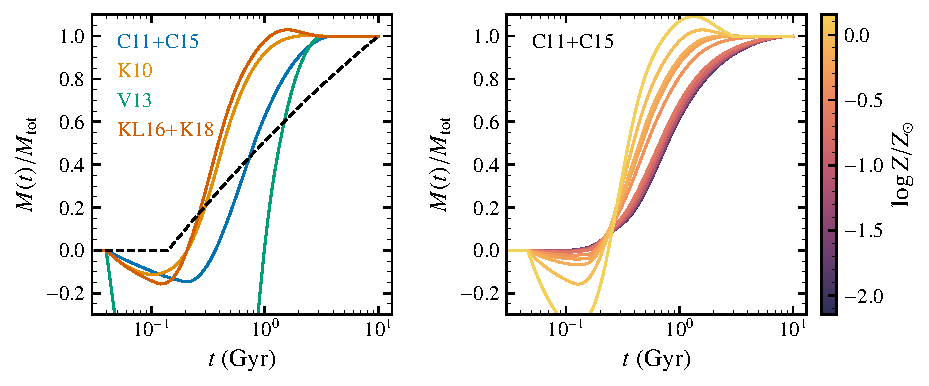
\includegraphics[scale=1]{y_agb_t2.pdf}

    \caption[AGB yields delay time distribution]{
        C production by AGB stars as a function of SSP age, normalized to the total mass $M_{\rm tot}$ produced at $t=10$ Gyr. Left: The four AGB yield models from literature at solar metallicity (C11, K10, V13, or K16). The delay time distribution of type Ia supernovae ($\propto t^{-1.1}$) is plotted as a dashed black line for comparison. Right: The C11 AGB model at different metallicities. }
    \label{fig:agb-ssp}
\end{figure}


Fig.~\ref{fig:yagb-z} shows IMF-averaged C yields for each AGB model as a function of metallicity $Z$.
V13 differs in that it shows a non-monotonic metallicity dependence. However, this effect is only for models with $\log Z/Z_\odot \lesssim -1$.
Otherwise, models differ only in their yield normalization and metallicity dependence. All models predict yields within a factor of \about{2} for fixed metallicity.
For example, the three models C11, K10, and K16 predict $y_\text{C}^\text{AGB}$ to be between 0.006 and 0.008 at solar metallicity, but C11 has a much shallower metallicity dependence than the K10 and K16 models. V13 instead predicts a yield \about{0.004}.

\begin{figure}
    \centering
    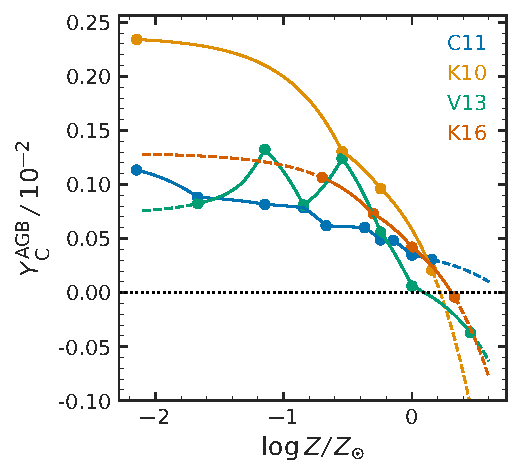
\includegraphics[scale=1]{y_agb_vs_z.pdf}

    \caption[AGB yield metallicity dependence]{The net fractional IMF-weighted AGB C yield $\Ycagb$ as a function of metallicity for each of our AGB yield models.
    }
    \label{fig:yagb-z}
\end{figure}

\section{Core Collapse Supernovae}


Massive stars form $^{12}$C in their cores through the triple--$\alpha$ process. However, only C ejected through supernovae and stellar winds contributes to the yield. 
While there are many stellar models providing predictions of CCSNe yields, the results of these models are highly uncertain due to the many stellar modeling uncertainties. 

In Fig.~\ref{fig:y_cc}, I plot calculations of the IMF-integrated yields, defined with Eq.~\ref{eq:imf-yield} (computed using \VICE's \texttt{vice.yields.ccsne.fractional} function). 
CCSNe models predict a wide range of C yields, spanning almost 1 dex. 
Both the \citet{NKT13} and \cite{LC18} models show positive metallicity dependence. 
The \cite{LC18} models also include rotation, showing that variations in the rotational velocity of the star can dramatically increase C production and the metallicity dependence of $\Ycc$. Rotation induces more mixing allowing the CO core to grow larger. Our fiducial model's steep metallicity dependence near $Z\approx Z_\odot$ could be explained by rotation. 
Fig.~\ref{fig:y_cc} shows the C11 model for comparison on the top. Especially at $Z\approx Z_\odot$, most CCSNe models dominate AGB C production. I will later also show empirically that CCSNe should dominate C production. 

On the bottom of Fig.~\ref{fig:y_cc}, I also show the CCSNe-[C/Mg] ratio, defined by
\begin{equation}\label{eq:c_mg_cc}
    {\rm [C/Mg]^{CC}} = \log_{10}\left( \frac{\Ycc}{\Yoc}\right) - \log_{10} \left( \frac{Z_{{\rm C},\ \sun }}{Z_{{\rm Mg},\ \sun }} \right).
\end{equation}
${\rm [C/Mg]^{CC}}$ describes what [C/Mg] would be if CCSNe were the only process producing C.
Once again, different CCSNe models span a large range in [C/Mg]. 
I chose to instead parameterize $\Ycc$ to enable agreement with observations, as most CCSNe models fail to achieve near-solar [C/Mg].
Assumptions about the explodability landscape affect C and Mg production. Increasing the fraction of stars that explode increases $\Ycc$, as stars that directly collapse do not contribute to explosive yields \citep{emily+21}. However, C is relatively unaffected by the black-hole landscape, as very massive stars contribute carbon through enriched winds. Since Mg is formed deeper in the core of massive stars, the Mg yield drops much more steeply, so models, where few stars explode (S16/W18), result in much higher [C/Mg].

CCSNe models also do not reach [O/Mg] due to overproduction of O, or underproduction of Mg, or both \citep{emily+21}. Here, I assume ${\rm [O/Mg]} = 0$, which is not compatible with CCSNe models but is consistent with APOGEE observations \citep{weinberg+19, weinberg+22}.
    

\begin{figure}[htp]
    \centering
    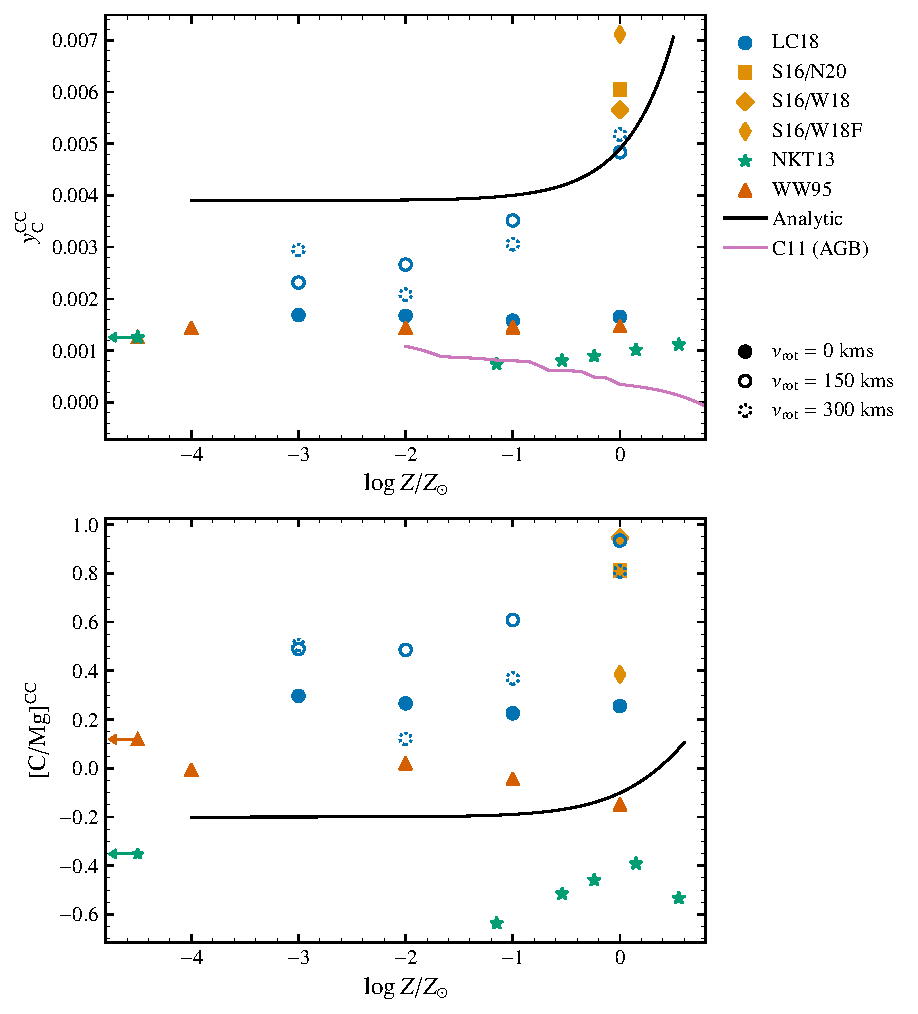
\includegraphics{y_c_cc.pdf}
    \caption[CCSNe C yields]{
        C yields from massive stars.
        \textbf{Top:} The IMF-weighted CCSNe yield of C as a function of metallicity.
        \textbf{Bottom:} The CCSNe [C/Mg] abundance ratio, defined in Eq.~\ref{eq:c_mg_cc}. The black line represents the C yield of the fiducial model,
    $\Ycc = 0.0028 + 0.001 (Z/Z_{\odot})$. Yields are shown for tables from 
    \citet[red triangles]{WW95}, \citet[orange squares and diamonds]{sukhbold+16}, 
    \citet[green stars]{NKT13}, and \citet[blue circles]{LC18}. \citet{sukhbold+16} report yields for different black hole landscapes, while \citet{LC18} provide yields at different rotational velocities.
In the top panel, the pink line denotes $\Ycagb$ from C11 for comparison.
}
    \label{fig:y_cc}
\end{figure}

\chapter{The Equilibrium Approximation}\label{sec:equilibrium}

In the presence of metal-poor gas accretion and feedback-driven outflows, galaxies reach an equilibrium abundance in which production of new metals is balanced by losses to new stars and outflows \citep{larson72, dalcanton07, FD08, PS11, lilly13}.
While our galaxy is likely not in perfect equilibrium or described by a single, homogeneous chemical region, the equilibrium approximation is nevertheless useful in understanding yields and metallicity dependence \citep[e.g.][]{james_dwarf,james+23,WAF17}. 

I assume a simple ``one-zone'' chemical evolution model \cite[e.g.][]{tinsley80, pagel09, matteucci21}.  Newly produced metals are homogeneously and instantaneously mixed, so spatial dependence is neglected.
I define $M_{X}$ to be the mass of element X in the gas phase, $\dot{M}_\star$ to be the star formation rate (in M$_\odot$ yr$^{-1}$), and $\eta$ to be the mass loading factor $\eta\equiv\dot{M}_{\rm outflow}/\dot{M}_\star$ (representing the strength of outflows).
SSPs return a fraction $r$ of their birth mass back to the ISM, due to ejected stellar envelopes. ($r\approx0.4$ for a \citealt{kroupa01} IMF.)
Given the IMF-averaged yield of Mg $y_{\rm Mg}$, the rate of change in the ISM mass of Mg $\dot{M}_{\rm Mg}$ is a simple sum of sources and sinks,
\begin{equation}
    \dot{M}_{\rm Mg} =  y_{X}\dot{M}_\star - \dot{M}_{\rm Mg~remnants} - \dot{M}_{\rm Mg,~outflows},
\end{equation}
where the first term on the right-hand side describes CCSNe enrichment. 
In terms of the return mass fraction of stars $r$, the mass lost to remnants is $Z_X (1-r)\dot{M}_\star$.  And, the outflows deplete mass at a rate $Z_X \eta\dot{M}_\star$. ( I assume the composition of outflows is the same as the ISM.) Substituting for $\eta$ and $r$,  
\begin{equation}
    \dot{M}_{\rm Mg}= y_{X} \dot{M}_\star - (1 + \eta - r) Z_{X} \dot{M}_\star.
\end{equation}
Assuming an exponentially declining star formation history $\dot{M}_\star \propto e^{-t/\tau_{\rm sfh}}$, the equilibrium abundance is derived analytically by setting $\dot{Z}_{Mg}=0$.
\begin{equation}\label{eq:z_eq}
    Z_{\rm Mg}^{\rm eq}(R) = \frac{y_{\rm Mg}}{1 + \eta(R) - r - \tau_\star / \tau_{sfh}},
\end{equation}
where $\tau_{\star}$ is the star formation rate.
In the special case of constant star formation, $\tau_{\rm sfh}\to\infty$, the denominator simplifies to $1+\eta-r$.

While Equation \ref{eq:z_eq} can be applied to CCSNe C, the delayed nature of AGB C can complicate the expression. Instead, I use an effective yield, which can be expressed as an integral over the DTD,
\begin{equation}
    \langle \Ycagb\rangle = \frac{\int_0^T \tilde{y}_{\rm C}^{\rm agb}(M, Z) \dot{M}_\star(T - t) \frac{dN}{dM} \frac{dM}{dt} dt  }{ \dot{M}_\star \int_0^T \frac{dN}{dM} \frac{dM}{dt} dt}.
\end{equation}
Eq.~\ref{eq:z_eq} then becomes
\begin{equation}
    Z_{\rm C}^{\rm eq}(R) = \frac{\Ycc + \langle\Ycagb\rangle}{1 + \eta(R) - r - \tau_\star / \tau_{sfh}}
\end{equation}
And the equilibrium C/Mg abundance ratio is
\begin{equation}\label{eq:z_co}
    \frac{Z_{\rm C}^{\rm eq}}{Z_{\rm Mg}^{\rm eq}} = \frac{\Ycc + \langle \Ycagb \rangle }{\Yoc}.
\end{equation}
Analogous to \cite{james+23} arguments about N, the trends in abundance ratios are set by yield ratios in these GCE models. The effect of other GCE parameters (most importantly $\eta$) cancels. As a consequence, yield ratios should establish abundance ratio trends in models which assume a different normalization of element yields and mass-loading (see discussion below).
This argument can also be inverted to infer  yields from abundance ratio trends. To the extent that observed C and Mg trends reflect the equilibrium abundances in different Galactic regions, we can infer the CCSNe yield given an assumed AGB star yield (or vice versa). Inferring $\Ycc$ from $\Ycagb$, 
\begin{equation}
    y_\text{C}^\text{CC} =  y_\text{Mg}^\text{CC} \frac{Z_\text{C,~eq}}{Z_\text{Mg,~eq}} - \langle y_c^{agb} \rangle
\end{equation}
Rewriting this expression as a relative yield of C and Mg,
\begin{equation}\label{eq:y_c_eq}
    \frac{\Ycc}{\Yoc} = \frac{Z_{\text{C},~\odot}}{Z_{\text{Mg},~\odot}} 10^{\rm [C/Mg]} - \frac{\langle \Ycagb \rangle}{\Yoc}.
\end{equation}

\section{Yield Models}

As I will discuss in \S\ref{sec:outflows}, the normalization of yields and $\eta$ is degenerate. This can be observed in Eq.~\ref{eq:z_co}, where changes in $\eta$ or the scaling of $y_{\rm C}/y_{\rm Mg}$ would not affect equilibrium trends. Furthermore, in Eq.~\ref{eq:z_eq}, an increase in both $y_{\rm Mg}$ and $\eta$ would leave $Z_{\rm Mg}^{\rm eq}$ unchanged. My models here are unable to distinguish the overall scaling of yields and outflow mass loading, and choosing to keep $y_{\rm C}$ fixed reduces unnecessary free parameters. 
%
As a result, I choose to leave the total carbon yield fixed at solar $Z$,
\begin{subequations}
    \begin{align}
        \Yct~\big\vert_{Z=Z_\odot} &= \Ycc + \Ycagb = 0.005 \\
        \Yct/\Yoc~\big\vert_{Z=Z_\odot} &= 2.7.
    \end{align}
\end{subequations}
This ratio results in an equilibrium abundance ${\rm [C/Mg]} = -0.09$, which is consistent with the \citetjack~subgiant sample and is within \about{20\%} of the solar C/Mg mixture from \citet{asplund+09}.

In \S\ref{sec:f-z-models}, I will show that none of the four AGB yield sets (C11, K10, V13, K16) produce enough C relative to this $\Ycc$ value. So, I introduce normalization factors, $\alpha_{\rm AGB}$, and $\alpha_{\rm CC}$ which denote a multiplicitave scaling of $\Ycc$ and $\Ycagb$ respectively. 
\begin{subequations} \label{eq:alpha}
    \begin{align}
        \Ycagb &\rightarrow \alpha_{\rm AGB} \left(\Ycagb\right) \\
        \Ycc &\rightarrow \alpha_{\rm CC} \left(\Ycc\right)\\
        \alpha_{\rm CC} &= \frac{\Yct - \alpha_{\rm AGB} \left(\Ycagb\right)}{\Ycc}
    \end{align}
\end{subequations}
Above, $\alpha_{\rm CC}$ is dependent on the choice of $\alpha_{\rm AGB}$ to keep the total carbon yield constant. 

In \S\ref{sec:f-z-models}, I find that $\alpha_{\rm AGB}\approx 2.9$ for the C11 yield model. Using this AGB yield, I can now use Eq.~\ref{eq:y_c_eq} to find an estimate of $\Ycc$ as a function of metallicity. I show the values of $\Ycc$ I obtain from the subgiant sample in Fig.~\ref{fig:analytic}. From regression analysis, I suggest here that
\begin{equation}
    \Ycc = 0.0028 + \zeta\left(\frac{Z}{Z_\odot}\right),
\end{equation}
where $\zeta$, describing the metallicity dependence, is $\zeta\approx0.001$.


\begin{figure}
    \centering
    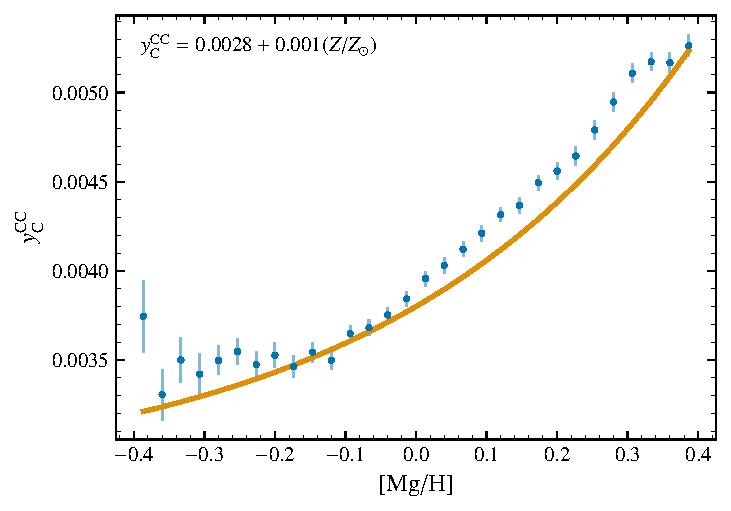
\includegraphics[]{analytic.pdf}
    \caption[Reverse fit yields]{Inferred massive star C yields as a function of metallicity. I assume equilibrium and $3\times {\rm C11}$ AGB yields (orange curve, see discussion in Section \ref{sec:equilibrium}). The binned medians and median absolute deviation (divided by $\sqrt{N}$) are blue points.
    }
    \label{fig:analytic}
\end{figure}





\section{Uncertainties}

I only perform this analysis on the C11 yields because C11 has yields tables more finely sampled in metallicity than the other three AGB yield tables. As the metallicity range of the data is small ($-0.4\lesssim {\rm [Mg/H]} \lesssim 0.4$), other models are more challenging to interpret in this range. Furthermore, the APOGEE observations may have systematics, and other measurements of C abundances \citep[e.g.][]{vincenzo+21} have slight disagreements in the overall shape of the trend (see \S\ref{sec:jack}).
So, this expression of $\Ycc/\Yoc$ depends on the chosen AGB yield table, the AGB fraction, and the dataset. 
Additionally, these yields will be systematically biased if the galaxy is out of equilibrium, for example due to a recent starburst (Isern et al. 19; Mar et al. 19). Further exploration could investigate the magnitude of these uncertainties, but I find that the qualitative conclusions are similar despite substantial variations in the assumptions here.



\chapter{The Multizone Model}\label{sec:vice}

Classical, ``one-zone'' models of chemical evolution assume instantaneous mixing of metals in the star-forming ISM \citep[e.g.][]{matteucci21}. This simple framework is a poor approximation for the Milky Way.  The Galaxy evolves ``inside out''---where star formation is higher towards the center and in the early universe \citep{bird+13}. Additionally, stars can migrate several kpc over their lifetimes, mixing together different chemical environments across the galaxy \citep{bird+12,sellwood+binney02}. For the rest of this paper, I focus on multizone models, which discretize the Galaxy into concentric annuli and allow stars to move between rings.  Specifically, I make use of the \citet{james+21} (hereafter \JJ) model for the Milky Way, which runs using the publicly available Versatile Integrator for Chemical Evolution (\VICE). This model is described extensively in \JJ~and concisely summarized  in \citet{james+23}. Here, I provide a brief overview of the relevant model components.

In the model, the Galaxy is divided into 200 rings, each 100 pc wide. Each ring has a separate stellar population and gas supply. Star formation ends beyond a radius $R=15.5$ kpc. I initially assume an ``inside-out'' Star Formation History (SFH), where the star formation surface density $\Sigma_\star$ is given by 
\begin{equation}
    \dot{\Sigma}_\star \propto \left(1-e^{-t/\tau_{\rm rise}}\right) e^{-t/\tau_{\rm sfh}}.
\end{equation}
$\tau_\text{rise}=2$ Gyr describes when the star formation rate reaches a maximum, and $\tau_{\rm sfh}$ describes the decay timescale of star formation as a function of radius $R$. \JJ~derives $\tau_{\rm sfh}(R)$ through analysis of four integral field spectroscopy surveys in \cite{sanches20}. The star formation history is normalized such that the total stellar mass reaches $M_\star=5.17\times10^{10} {\rm M}_\odot$ \citep{LM15} and at each $R$ to match the stellar surface density gradient \citep{BHG16}.
The gas inflow is calculated to maintain our chosen SFR for each radius and time. The gas-SFR law is based on an extension of a Kennicutt-Schmidt law \citep{kennicutt98}, motivated by 
\begin{equation}
\dot{\Sigma}_{\star} \propto \\
\begin{cases}
    {\Sigma}_{\rm gas} & 2\times 10^7 \leq \Sigma_{\rm gas} \\ 
    {(\Sigma}_{\rm gas})^{3.6} & 5\times 10^6 \leq \Sigma_{\rm gas} < 2\times10^7 \\ 
    {(\Sigma}_{\rm gas})^{1.7} & \Sigma_{\rm gas} < 5\times10^6 \\ 
\end{cases}
\end{equation}
The scaling of this relationship varies with time due to the redshift dependence of $\tau_\star$ in molecular gas observed by \citet{tacconi18}. I assume a Kroupa IMF \cite{kroupa01}.


\JJ\ accounts for radial migration by using the results of the \texttt{h277} hydrodynamical simulation \citep{christensen12, zolotov12, loebman12, BZ14}, with simulation parameters described in \citet{bird+21}. Each \VICE single stellar population (SSP) is matched to an \textit{analog} in \texttt{H277}, chosen to form at a similar time and radius $R$. By taking the change in radius $\Delta R$ of the analogs, the SSP move to their final radii with a $\sqrt{\text{time}}$ dependence.
This relationship between displacement and time arises when migration proceeds as a consequence of the diffusion of angular momentum \citep{frankel18, frankel20}.
I do not account for radial gas flows.
Using the results of a hydrodynamical simulation without modification limits the free parameters in the model; however, I am limited to one dynamical history. The impact of the details of a galaxy's dynamical history on its chemical evolution is unknown, and I do not explore this question here.

As the strength of outflows controls the resulting $\alpha$ abundances, \JJ~create a metallicity gradient by defining
\begin{equation}
\eta(R) = \frac{y_{\alpha}^{\rm CC}}{Z_{\alpha, \odot}} 10^{(-0.08\text{ kpc}^{-1})(R-4\text{ kpc})+0.3} + r - 1.
\end{equation}
This choice of $\eta(R)$ results in a [$\alpha$/H] gradient consistent with Milky Way observations \citep[e.g.][]{hayden+14, weinberg+19, frinchaboy+13}.


\chapter{Multizone Model Results}
\section{Data Selection}

\citet{james+23} compare their model against the \cite{vincenzo+21} sample of APOGEE \citep{apogee17} red giants whose C and N abundance have been corrected for mixing process using MESA stellar evolution models. 
I instead use the \citetjack~sample of APOGEE subgiants. Subgiant stars have not undergone FDU, so their atmospheric C and N abundances are still reflective of their birth abundances and do not need mixing corrections. I additionally only compare the models to the low-$\alpha$ sequence.  The selection criteria and differences between the samples are described in more detail in Appendix \ref{sec:jack}.



\section{The Evolution of C Abundances in the Galaxy}

Here, I present the time evolution of our fiducial model. In the next sections, I will discuss the choice of parameters and agreement with observations. 
The fiducial model has the following qualitative characteristics of its C yields: (a) C is predominantly produced in CCSNe, (b) CCSNe produce more C at higher metallicities, and (c) AGB stars produce less carbon at higher metallicities. Our fiducial model uses the C11 AGB yield tables (see \S\ref{sec:agb}, and Table \ref{tab:fiducial_mod}), and I amplify the C11 yields by a factor of 2.9 such that AGB stars account for 20\% of carbon at $Z=Z_\odot$. 

I show the time evolution tracks of the fiducial model in Fig.~\ref{fig:c_evo} for \caah~ and \caafe~. Comparing [C/$\alpha$] against [Mg/Fe] enables us to see the late-time evolution of C more clearly. Because of the extended DTD of SNeIa enrichment, [Fe/H] takes longer to reach equilibrium as half of Fe production comes from type-Ia supernovae, and the late time evolution is not as clustered as [$\alpha$/H].
The evolution proceeds as follows.
Initially, CCSNe dominate production. As $\Ycc$ has strong metallicity dependence, [C/Mg] increases with time. Shortly thereafter, AGB stars contribute delayed C, increasing [C/Mg] even more steeply. As Mg begins to reach equilibrium, the [C/Mg] ratio plateaus as C approaches equilibrium. Finally, as $\Ycagb$ decreases or even becomes negative with higher metallicity, the [C/Mg] abundance may decline slightly. 

This is even more evident in the lower panel of Fig.~\ref{fig:c_evo}. While the \caah~trend reaches equilibrium at \about{5} Gyr, the \caafe~trend continues to evolve even until the present day, exposing the effect of the relative delay times of AGB stars and SNeIa.


\begin{figure}
\centering
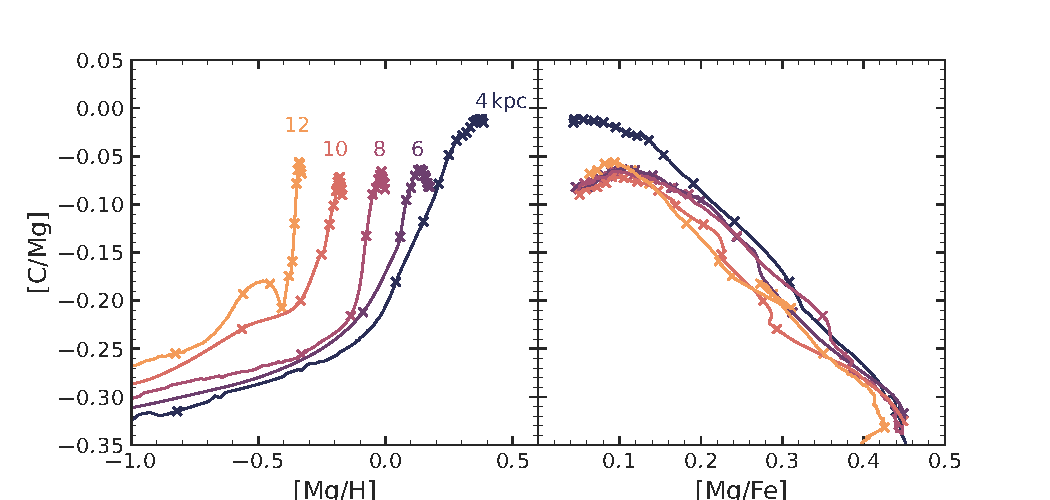
\includegraphics{evo_tracks.pdf}
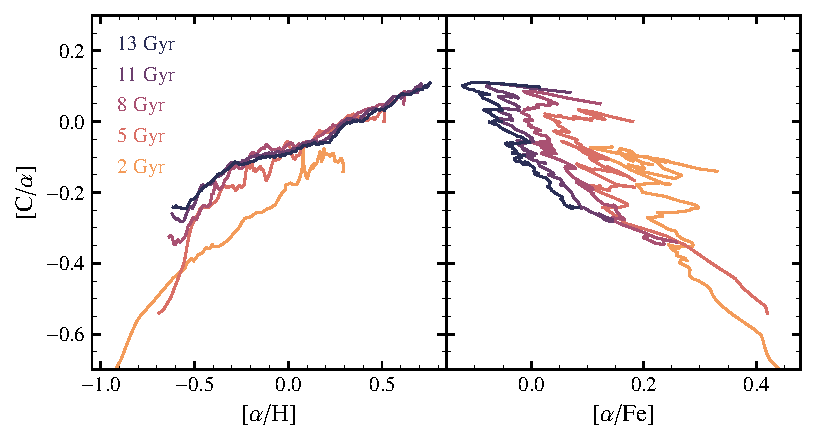
\includegraphics{evo_slices.pdf}
\caption[C chemical evolution tracks]{
    Time evolution of gas phase C abundances in our fiducial model.

    Top: Evolutionary tracks parameterized by time at fixed Galactocentric radius in the \caah and \caafe planes. 

    Bottom: snapshots of the gas-phase \caah~and \caafe~trend, parameterized by radius at a fixed time.
}
\label{fig:c_evo}
\end{figure}

\section{Alternate Models}\label{sec:f-z-models}

In Fig.~\ref{fig:agb_sims}, I compare the K10, K16, C11, and V13 yield models. Each model uses the published, unscaled yield tables. As the highest AGB yield at solar, K10 is only $\Ycagb=0.000585$, $f_{\rm AGB} \leq 0.12$ for all models. Massive stars dominate C production with unscaled yields.  While it is easy to modify the AGB yields in my model, their small contribution reduces the effect. I leave a more detailed discussion of the effects of AGB models for Appendix \ref{sec:alt_agb} and use C11 yields hereafter.

\begin{figure}
\centering
\includegraphics{oob_agb.pdf}
\caption[AGB GCE Models]{
    Stellar abundance trends in our model, assuming metallicity independent $\Ycc$. Colored lines quantify the median [C/Mg] in bins of [Mg/H] for our four AGB yield models from the literature (see \ref{sec:agb}). Black points and grey dashes represent the median and standard deviations in the \citetjack~sample. In the right panel, I show the trends only for stars where $-0.15\leq {\rm [Mg/H]}\leq -0.05$.
}
\label{fig:agb_sims}
\end{figure}



Next, I investigate adjustments to the AGB yield fraction $f_{\rm AGB}$ and the CCSNe metallicity dependence $\zeta$ in Fig.~\ref{fig:beta_f}. On the top panel of Fig.~\ref{fig:beta_f}, I plot models with varying $\Ycc$ metallicity dependence. As discussed in \S\ref{sec:equilibrium}, the \caah~trend is approximated by equilibrium, so the trends of these have steeper \caah~corresponding to steeper metallicity dependence. However, \caafe~is minimally affected by these changes since CCSNe are instantaneous in this model.

Now, I vary the proportion of AGB contribution.  The AGB C production fraction is defined as
\begin{equation}
    f_{\rm AGB} \equiv \frac{\Ycagb}{\Yct}\Bigg\vert_{Z=Z_\odot},
\end{equation}
where  $\Ycagb$ includes the multiplicative factor $\alpha_{\rm AGB}$ as defined in Eq.~\ref{eq:alpha}.
In the bottom panel of Fig.~\ref{fig:beta_f}, I plot three models with different AGB fractions while using C11 yields.  The \caafe~relationship is set by $f_{\rm AGB}$ because a specific amount of C must be released at a delayed time in order to match the SNeIa production of Fe and increase [C/Mg] as [Mg/Fe] decreases to reproduce the data.
Increased $f_{\rm AGB}$ results in a decreased slope in \caah, owing to the negative metallicity dependence of $\Ycagb$. So while \caah~alone cannot differentiate models which vary $f_{\rm AGB}$ and $\zeta$ correspondingly, \caafe~provides information on $f_{\rm AGB}$. So, I can use \caafe~to estimate $f_{\rm AGB}\approx 0.2$, and then choose $\zeta$ in order to match \caah.

One source of theoretical uncertainty in this result is that the SNeIa yield and DTD have their own uncertainties. I discuss variations in $y_{\rm Fe}^{\rm Ia}$ in Appendix \ref{sec:alt_agb}, and find that the qualitative conclusions are largely unaffected. I therefore focus on the choices of $y_{\rm Fe}^{\rm Ia} = 0.00214$ choices from the fiducial model here.

So, the scaling of the trend and metallicity dependence of C (as seen in
the \caah~trend) gives information on the total C yield and the behavior of CCSNe (as the dominating producer of C); the \caafe trend exposes the delayed effect of C from AGB contribution.

\begin{table}
	\centering
    \caption[AGB net solar IMF yields]{For each AGB yield set, our calculation of the effective SFH- and IMF-weighted C AGB yield, along with the multiplicative factor reaches an AGB contribution of 20\%.}
	\label{tab:alpha_agb}
	\begin{tabular}{lcr} % four columns, alignment for each
		\toprule 
		AGB Model & $y_{\rm C, 0}^{\rm AGB}$ & $\alpha_{\rm AGB, 20}$\\
        \midrule
		C11 & 0.000347 & 2.9\\
		K10 & 0.000585 & 1.7\\
		V13 & 0.000060 & 16.5\\
		K16 & 0.000421 & 2.4\\
		\bottomrule
	\end{tabular}
\end{table}


\begin{figure}
\centering
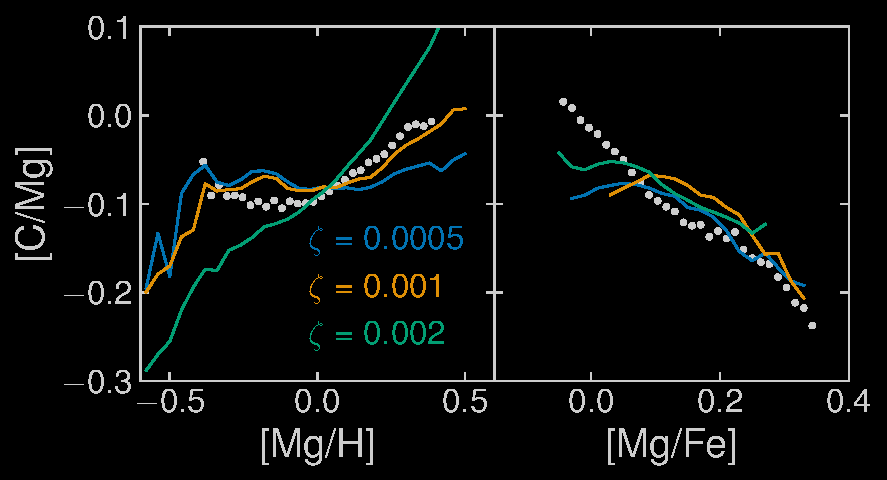
\includegraphics{beta.pdf}
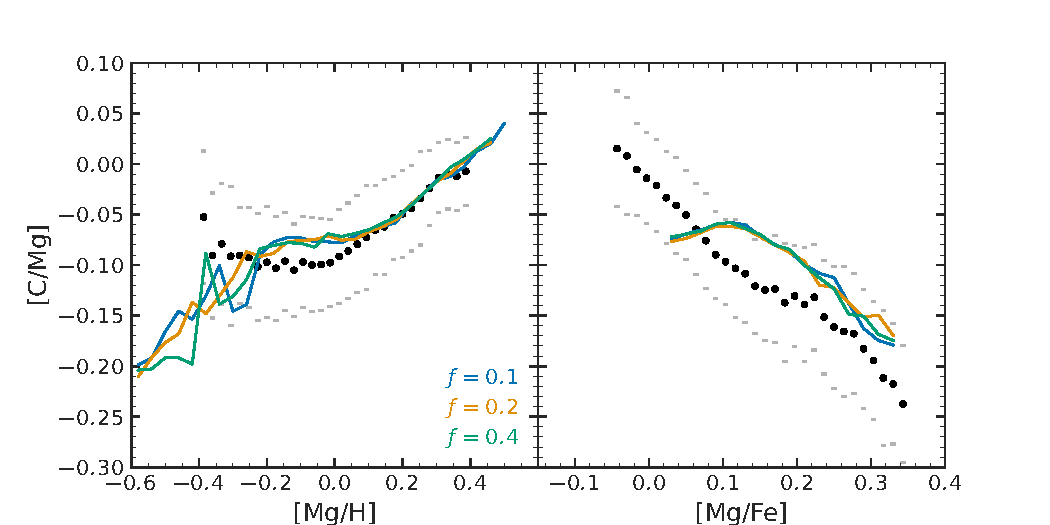
\includegraphics{f_agb.pdf}

\caption[Adjusted yield models]{Similar to Fig.~\ref{fig:agb_sims} except the top plot shows the fiducial model with lower and higher values of $\zeta$, the C-CCSNe metallicity dependence. The bottom plot shows models with $f_{\rm AGB}=$0.1, 0.2, and 0.4. Both the $f_{\rm AGB}$ and $\zeta$ influence \caah, but only $f_{\rm AGB}$ has a significant impact on \caafe.}
\label{fig:beta_f}
\end{figure}



\section{Star Formation History} \label{sec:sfh}



\begin{figure}
\centering
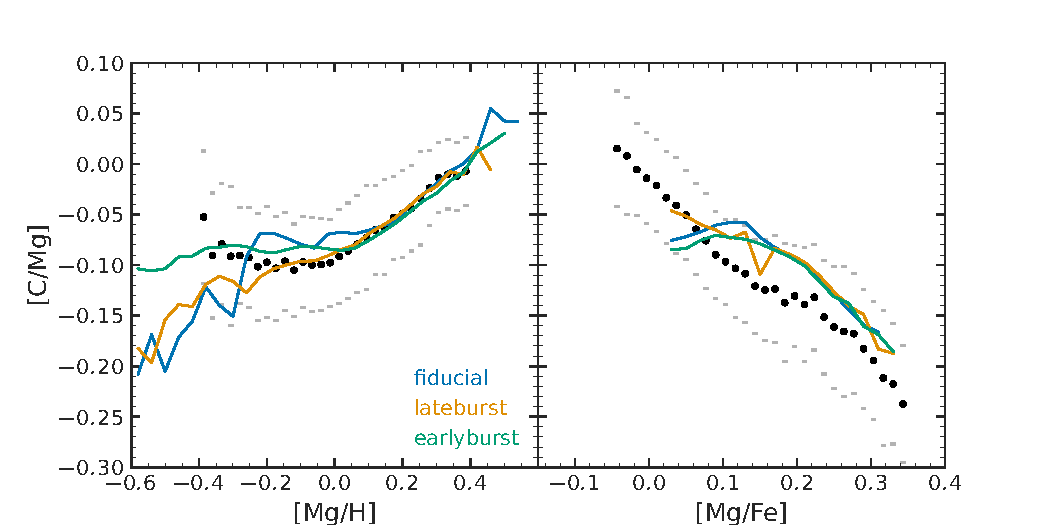
\includegraphics{lateburst_eta.pdf}

\caption[Lateburst models]{Same as Fig.~\ref{fig:agb_sims} but comparing the fiducial model to alternate star formation histories (see \S \ref{sec:sfh}).}
\label{fig:sfh_models}

\end{figure}


Here, I consider a "late burst" model, created by multiplying our fiducial "inside-out" SFH with a Gaussian.
\begin{equation}\label{eq:lateburst}
    \dot{\Sigma}_{\rm lateburst} \propto \dot{\Sigma}_{\rm insideout} \left(1 + A e^{-(t-\tau_{\rm burst})^2/2\sigma^2_{\rm burst}} \right)
\end{equation}

$A=1.5$ represents the amplitude of the birth, $\tau_\text{burst}=10.8$Gyr is the time where the burst is strongest, and $\sigma_\text{burst}=1$Gyr is the width of the burst.

I also consider an early burst model as a slight variation of the late burst, where the burst is instead exponential and placed at $t_1=5$ Gyr. This approximately corresponds to the Gaia-Encelidus merger, inducing higher star formation in the Milky Way \citep{spitoni21, bonaca20, helmi18}.
\begin{equation}\label{eq:twoinfall}
    \dot{\Sigma}_{\rm early-burst} \propto \dot{\Sigma}_{\rm insideout} + 
\begin{cases}
    Ae^{-(t-t_1)/\tau_{\rm burst}} & t_1 < t \\
      0 & t<t_1
\end{cases}
\end{equation}
where I take the burst duration, $\tau_{\rm burst}=1$ Gyr in this case. 

I show three models with these alternate SFH in Fig.~\ref{fig:sfh_models}. The changes to SFH leave \caah\ unchanged, but they do introduce slight variation in \caafe. Models with higher AGB fractions are more sensitive to variations in SFH. The late burst models result in [C/Mg] continuing to increase at low [Mg/Fe], but also introduce a break not present in the data. Additionally, the early burst
is able to reproduce the slight break between the low and high $\alpha$ sequences, but overshoots equilibrium more severely than the fiducial model. 
The choice of SFH does not change the large-scale slope of \caafe~significantly, so variations of SFH only have minimal effect on my conclusions.

\section{Outflows} \label{sec:outflows}

GCE models of the Milky Way fall into two classes---those which incorporate significant mass-loading (e.g., as in this work) and those which neglect mass-loading but lower effective yield to match observed abundances \citep{MCM13, MCM14, spitoni19, spitoni20, spitoni21}.
An increase in stellar yields has a nearly identical effect as a decrease in the mass-loading factor $\eta$ (see Appendix B of \cite{james_dwarf}).
The equilibrium arguments discussed in \S\ref{sec:equilibrium} suggest however that abundance ratios are independent of the choice of normalization and the value of $\eta$. I therefore expect my results regarding the relative yield $y_{\rm C}/y_{\rm Mg}$ and its metallicity dependence to extend to the other class of models omitting mass loading. I demonstrate this further here.

The theoretical motivation for decreasing yields is the uncertainty in stellar explodability.
If fewer massive stars explode, then the yields will be reduced by some factor. Additionally, some fraction of SN ejecta may be lost directly to an outflow, lowering effective yields. To explore reduced outflow models, I lower both $\eta$ and all yields by the same factor to leave the equilibrium abundances unchanged. 

\begin{figure}

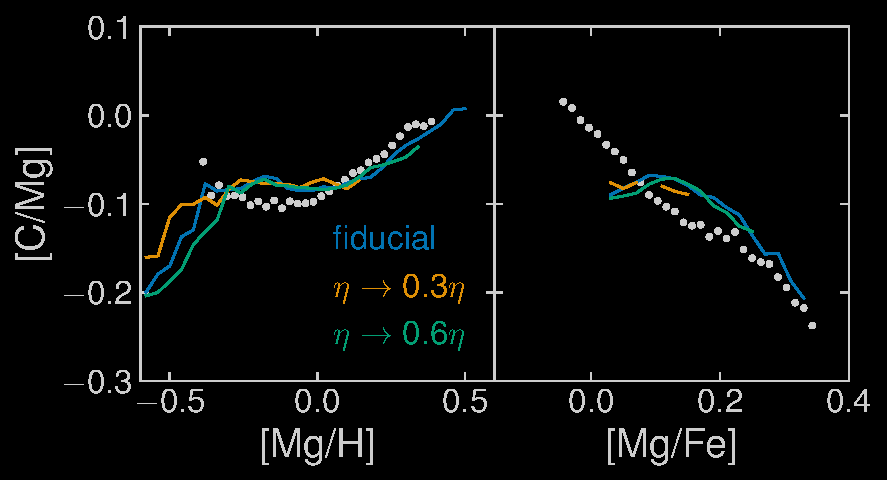
\includegraphics{eta.pdf}

\caption[Reduced-outflow models]{Same as Fig.~\ref{fig:agb_sims} but comparing the fiducial model to reduced outflow models (see \S \ref{sec:outflows}).}
\end{figure}


\section{Scatter}

Median trends have limitations as they do not consider the actual distribution of \caah~abundances. So, I show in Fig.~\ref{fig:scatter} a comparison of the predicted distribution of the model to the contours of the subgiant sample. Our model reproduces this 2-dimension distribution well when including scatter based on the median APOGEE abundance errors for each metallicity bin. Some of the scatter is due to radial migration, but observational errors are dominant. Precision abundance measurements will allow tighter constraints on chemical yields. 

\begin{figure}
    \centering
    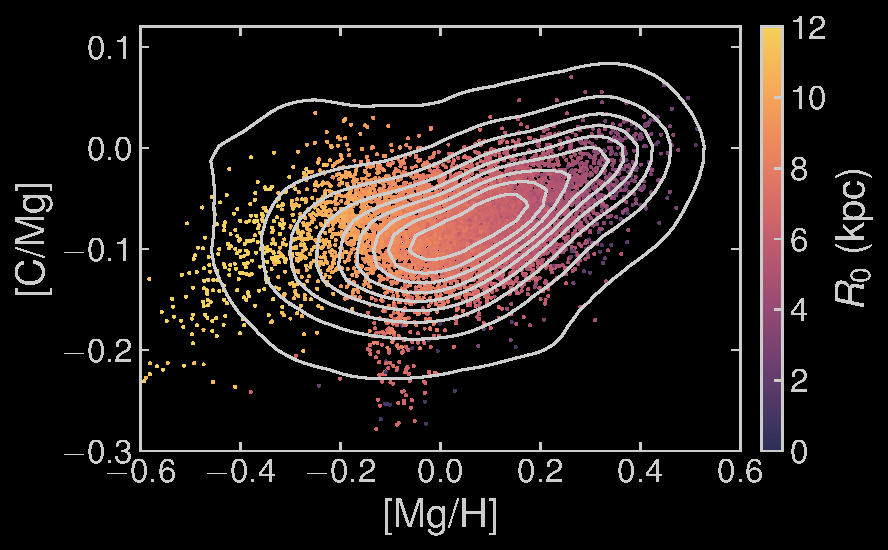
\includegraphics[scale=0.9]{cooh_scatter.pdf}
    \caption[Scatter agreement]{The stars in the fiducial model in the \caah~plane perturbed by the median [Mg/H] and [C/Mg] measurment errors in the \citetjack~sample. Stars are color-coded such that lighter colors represent populations born at greater galactocentric radii
    }
    \label{fig:scatter}
\end{figure}



\section{Gas-Phase C Abundances}\label{sec:gas}

As an additional test of the model, I next compare the gas-phase predictions against gas-phase C data. In Fig.~\ref{fig:gas_phase}, I plot our fiducial model's gas phase predictions compared to observations of MW and extragalactic HII regions, halo stars, and Damped Lyman Alpha (DLA) systems. The model is broadly consistent with observations, where the model at $t=2$ Gyr approximates the slope of dwarf galaxies and halo stars. The increase of C/O at late times is also consistent with the high C/O abundances measured in extragalactic HII regions. 
My model does not extend to very low metallicity, where the trend reverses, but broadly explains observations above $\rm [O/H] \sim -1$. 

Stellar measurements of Mg are more reliable, but O abundances are easier to measure in HII regions.  I therefore use Mg abundances from the \citetjack~subgiant sample as my primary empirical constraint. However, I use O abundances for gas-phase measurements and low-metallicity stars (\S \ref{sec:gas}). I model both Mg and O as metallicity-independent population-averaged yields dominated by massive stars. ${\rm [O/Mg]}\approx 0$ across a wide range of metallicities in APOGEE \citep{weinberg+19, weinberg+22}. 
I adopt O and Mg relative yields given by the solar mixture of \cite{asplund+09}.

C/O gas-phase measurements are hard. In HII-regions, C/O abundance ratios are measured with either recombination lines or collisionally excitation lines. However C lacks strong collisional excitation lines, and recombination lines fall in the ultraviolet without nearby reference H lines \citep{skillman+20}. Additionally, recombination and collisionally excitation measurements disagree by a factor of \about{2} \cite{GR07}.
Additional to measurement errors, variations in SFH may explain the scatter, as C contains delayed enrichment, and bursts cause variations in C/O. 

The decreasing [C/O] abundance at very-low metallicities is likely due to population III stellar yields \citep[e.g.][]{hirschi07}, as suggested by \citep{cooke+17, FN15}.
As AGB stars do have a significant delay, these stars cannot explain the increase in C yields at low metallicity as the timescales to reach $\rm [O/H]\sim -1$ is faster than this enrichment can occur. So, enhanced carbon due to (rotating) massive population III stars at low metallicities explains this trend.

\begin{figure}
    %\includegraphics{nitrogen.pdf}
    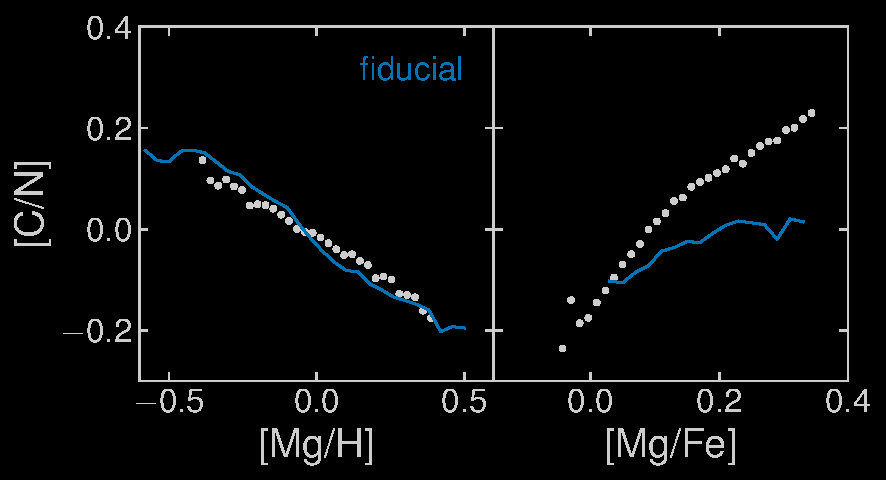
\includegraphics{c_n.pdf}
    \caption[C/N abundance agreement]{Similar to Fig.~\ref{fig:agb_sims}, except comparing [C/N] from the fiducial model only.
    }
\end{figure}

\begin{figure*}
\centering
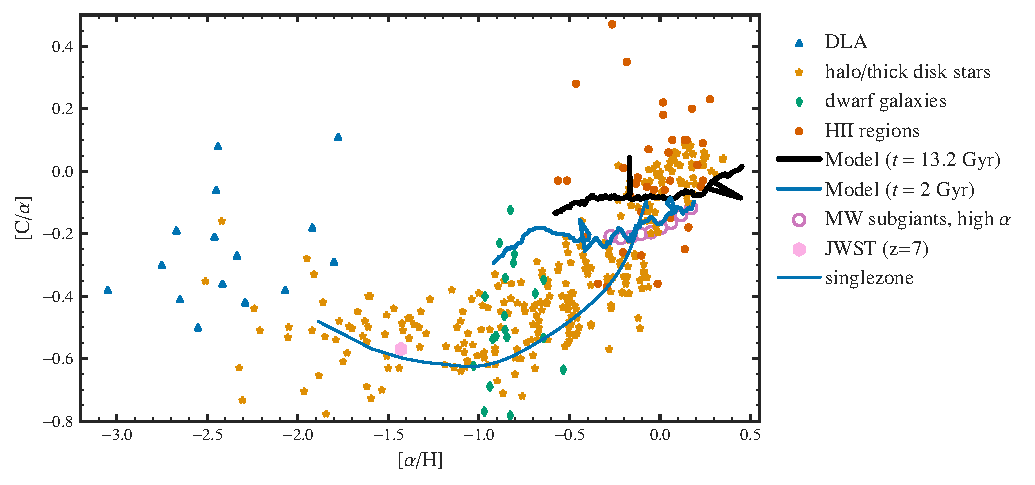
\includegraphics[]{summary.pdf}
\caption[Gas phase abundances]{Gas-phase C abundances. We plot our model at $t=2$Gyr and present day as thick solid lines. Points represent measurements in 
    HII regions    \citep[pink circles;][]{skillman+20, esteban+02, esteban+09, esteban+14, esteban+19}
    Damped Lynman-$\alpha$ (DLA) systems \citep[blue triangles;][]{cooke+17} 
    Milky Way halo and thick disk stars \citep[green stars;][]{nissen+14, fabbian+09}. 
    dwarf galaxies \citep[red diamonds;]{berg+19},
    and Milky Way high-$\alpha$ stars (yellow points; \citealtjack)
}
\label{fig:gas_phase}
\end{figure*}


\chapter{Conclusions}

In this work, I investigate the role of C yields on the predictions of multizone GCE models. \citet{james+23} performed a similar analysis focusing on N. They found that matching the observed relationship between N and O abundances (REFS) requires relative N and O yields from simple stellar populations with a roughly linear dependence on metallicity (i.e. $y_{\rm N}/y_{\rm O} \propto Z$). 
Here, I perform a similar analysis on C. 

Though CCSNe C yields are poorly understood, I adopt an equilibrium approximation and determine a functional form that approximately matches trends in APOGEE subgiants and is consistant with massive star nucleosynthesis models. Variations of the metallicity dependence of this CCSNe yield affect trends in \caah~but do not affect trends in \caafe\ when taking a slice in [Mg/H]. As all theoretical AGB C yields decrease with metallicity, increasing the AGB fraction causes the \caah\ trend to flatten. However, the \caafe\ trend is sensitive to the AGB fraction. 
From this, I estimate that AGB stars contribute \about{20\%} of total C abundance at solar metallicity. The remaining \about{80\%} of C comes from massive stars with a metallicity dependent yield of $\Ycc/\Yoc=1.51 + 0.54 (Z/Z_\odot)$. 
This metallicity dependence is consistent with the rotating stellar models of \citet{LC18}. 
 

I additionally explore variations of the assumed SFH and outflow mass-loading factor $\eta$. I find that alternate SFHs can slightly affect \caafe, but \caah~is mostly unaffected. Decreasing both outflows and yields by the same factor leaves the \caah~and \caafe~trends unaffected. These constraints on the relative yields of C, O, and Mg are robust against variations in $\eta$.

Finally, I compare my model against gas phase measurements and metal-poor stars. While my model was built on data near solar metallicity, observations of very low metallicity, high redshift damped Lyman-$\alpha$ systems indicate higher C/O ratios \citep{cooke+17}, consistent with yields from population III stars \citep[e.g.][]{hirschi07}. Our combined results self-consistently explain C abundances. 

These C yield constraints provide a useful benchmark for stellar evolution models. C yields are sensitive to poorly understood processes, including mass loss prescriptions, explodability, nuclear cross sections, convection, and stellar structure. Future spectroscopic surveys combined with Gaia kinematics \citep{gaia} will continue to enhance our understanding of chemical evolution. Both SDSS-V/MWM \citep{sdssv} and the DESI Milky Way survey \citep{desi, desi:mw} will each measure spectra of $>6$ million Milky Way stars. These larger samples will enable similar work to tighten constraints on stellar models and our understanding of galaxy structure and evolution.


%%%%%%%%%%%%%%%%%%%% REFERENCES %%%%%%%%%%%%%%%%%%

\newpage
\bibliographystyle{aasjournal}
\addcontentsline{toc}{chapter}{Bibliography}
\bibliography{main} 


%%%%%%%%%%%%%%%%% APPENDICES %%%%%%%%%%%%%%%%%%%%%

\appendix
\chapter*{Appendix}
\addcontentsline{toc}{chapter}{Appendix}
\renewcommand{\thesection}{A.\arabic{section}}
\renewcommand\thefigure{A\arabic{figure}}    
\renewcommand\theequation{A\arabic{equation}}    
\setcounter{figure}{0}
\setcounter{equation}{0}



\section{The APOGEE Subgiant Sample}\label{sec:jack}

I use the criteria outlined in \citetjack~to create a sample of subgiants from APOGEE DR17 \cite{apogee17} as our primary observational constraint. Subgiants are reflective of birth abundances for CNO \citep{souto19}. with chemical abundance determinations from ASPCAP \citep{aspcap}. SDSS 17 \cite{sdss17}.
\citetjack~select a region of stars in $\log g$-$T_\text{eff}$ space described by the following polyhedron
\begin{equation}
    \begin{cases} \label{eq:subgiant_selection}
        \log \text{g} \geq 3.5 \\
        \log \text{g} \leq 0.004T_{\rm eff} - 15.7 \\
        \log \text{g} \leq 0.000706T_{\rm eff} + 0.36 \\
        \log \text{g} \leq -0.0015T_{\rm eff} + 12.05 \\
        \log \text{g} \geq 0.0012T_{\rm eff} - 2.8 \\
    \end{cases}
\end{equation}

\begin{figure}
    \centering
    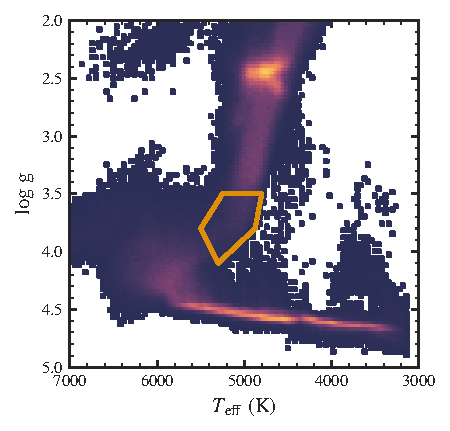
\includegraphics{logg_jack.pdf}
    \caption[Subgiant selection]{
        A Kiel diagram of APOGEE stars. Following \citetjack, we select subgiants in the orange polygon (see Equation \ref{eq:subgiant_selection}). These stars have not yet experienced first dredge-up, so their photospheric C and N abundances should reflect their birth mixture.
    }
\end{figure}

This cut isolates a clean sample of \about{12,000} subgiants. As first dredge up, which affects C and N abundances, only occurs during the ascent onto the red giant branch, subgiant stars are unaffected by this enrichment. 

Additionally, I included stars in APOGEE marked by the following flags.
\begin{itemize}
\item \verb|APOGEE_MIRCLUSTER_STAR|
\item \verb|APOGEE_EMISSION_STAR|
\item \verb|APOGEE_EMBEDDEDCLUSTER_STAR|
\item \verb|young cluster (IN-SYNC)|
\item \verb|APOGEE2_W345|
\item \verb|EB planet|
\end{itemize}

A second approach in determining birth abundances in stars is to correct the surface abundance effects of FDU, as in \cite{vincenzo+21}. I note that there is a slight difference in the yields found through \cite{vincenzo+21} and \citetjack. As o

\begin{equation}\label{eq:high_alpha}
\begin{cases}
\text{[Mg/Fe]} >0.12-0.13\text{[Fe/H]}, & \text{[Fe/H]}<0\\
\text{[Mg/Fe]} >0.12, & \text{[Fe/H]}>0\\
\end{cases}
\end{equation}

, discussion of GALAH C in \citealt{emily+19}).


I choose to use \citetjack's sample as this does not rely on additional layers of modeling, providing a more direct constraint to our model and limiting our systematic uncertainties.

\newpage
\section{Additional Considerations of Yields}\label{sec:alt_agb}

As I focus on constraining relative yields, I neglect O and Mg yield variations in the main text. There is substantial variation in Mg predictions (see Fig.~\ref{fig:y_mg}). Most models predict relatively flat Mg trends with metallicity (even with rotating models from \citealt{LC18}). However, the variation is significant and my adopted $\Yoc$ yield is much higher than most models. This is a known problem (see \citet{emily+21}). CCSNe models overpredict O or underpredict Mg, and the resolution is still unknown. 
My results are, however, independent of whether the CCSNe element is O or Mg.

While I focus the main discussion of the paper on the C11 model, other AGB models can impact abundance trends when $f_{\rm AGB}$ becomes larger.
Here, I briefly explore the effects of variations in AGB models that affect abundance trend predictions when these models are amplified to match observational [C/MG]-[Mg/Fe] trends. 
See Fig \ref{fig:fagb2}.

V13 is also interesting as at high metallicity, the yields quickly become strongly negative. This causes a reversal of the [C/Mg]-[Mg/Fe] trend at high [Mg/H] slices (figure ...). As our set of observations does not appear to reverse, this indicates that C yields are likely to stay positive even at slightly super-solar, so models like V13 are a poor match to observations. 

In Fig.~\ref{fig:fe_ia}.

I leave the exploration of the age-metallicity relation for C to future work.


\begin{figure}[htp]
    \centering
    \includegraphics{agb2.pdf}

    \caption[Alternate AGB models]{Same as Fig.~\ref{fig:agb_sims} except where $f_{\rm agb}=0.2$. When yields are amplified, chaos ensues.}
    \label{fig:fagb2}
\end{figure}


\begin{figure}
    \centering
    \includegraphics{y_mg.pdf}
    \caption[Magnesium CCSNe yields]{Same as the top panel of Fig.~\ref{fig:y_cc}, but for Mg. Our Mg yield choice is shown as a dashed line at the top
    }
    \label{fig:y_mg}
\end{figure}

\begin{figure}
    \centering
    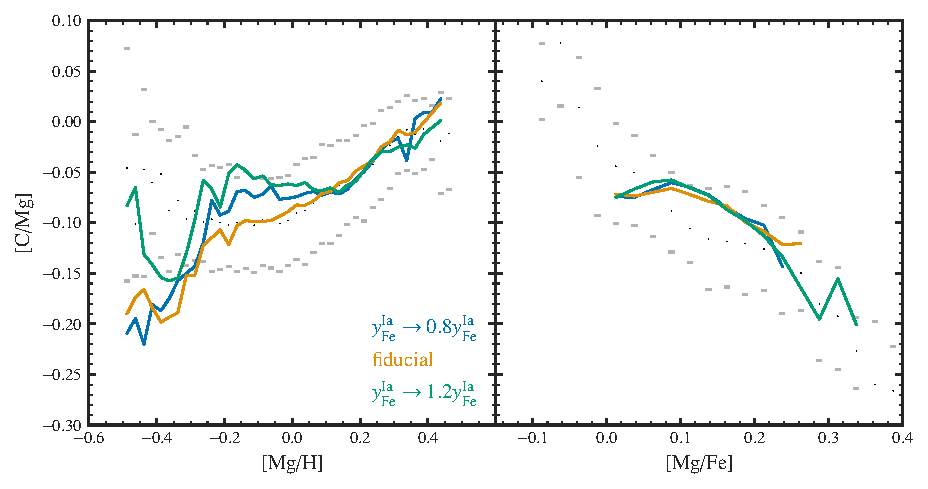
\includegraphics{fe_ia.pdf}
    \caption[Adjusting type Ia iron]{Similar to Fig.~\ref{fig:agb_sims} except with variations of the SNeIa iron fraction}
    \label{fig:fe_ia}
\end{figure}




\newpage

\section{Software}

Software that has contributed to this work:

\begin{itemize}
    \item \citet{OhioSupercomputerCenter1987}
    \item \VICE~\citep{JW20, james+21}
    \item \texttt{matplotlib} \citep{matplotlib}
    \item \texttt{scipy} \citep{scipy}
    \item \texttt{IPython} \citep{ipy}
    \item \texttt{pandas} \citep{pandas}
    \item \texttt{numpy} \citep{numpy}
    \item \texttt{astropy} \citep{astropy:2013, astropy:2018, astropy:2022}
    \item \texttt{seaborn}
\end{itemize}



\end{document}




